%% source: 2023-sp-midterm_02
%% tags: [depth first search]
\begin{prob}

    Suppose we define a \textit{forward-looking} graph with $n$ nodes to be the
    directed graph $G = (V, E)$ with nodes $u_1, \ldots, u_n$ and the edge
    $(u_i, u_j)$ if and only if $i < j$. An example of such a graph with 4
    nodes is shown below.

    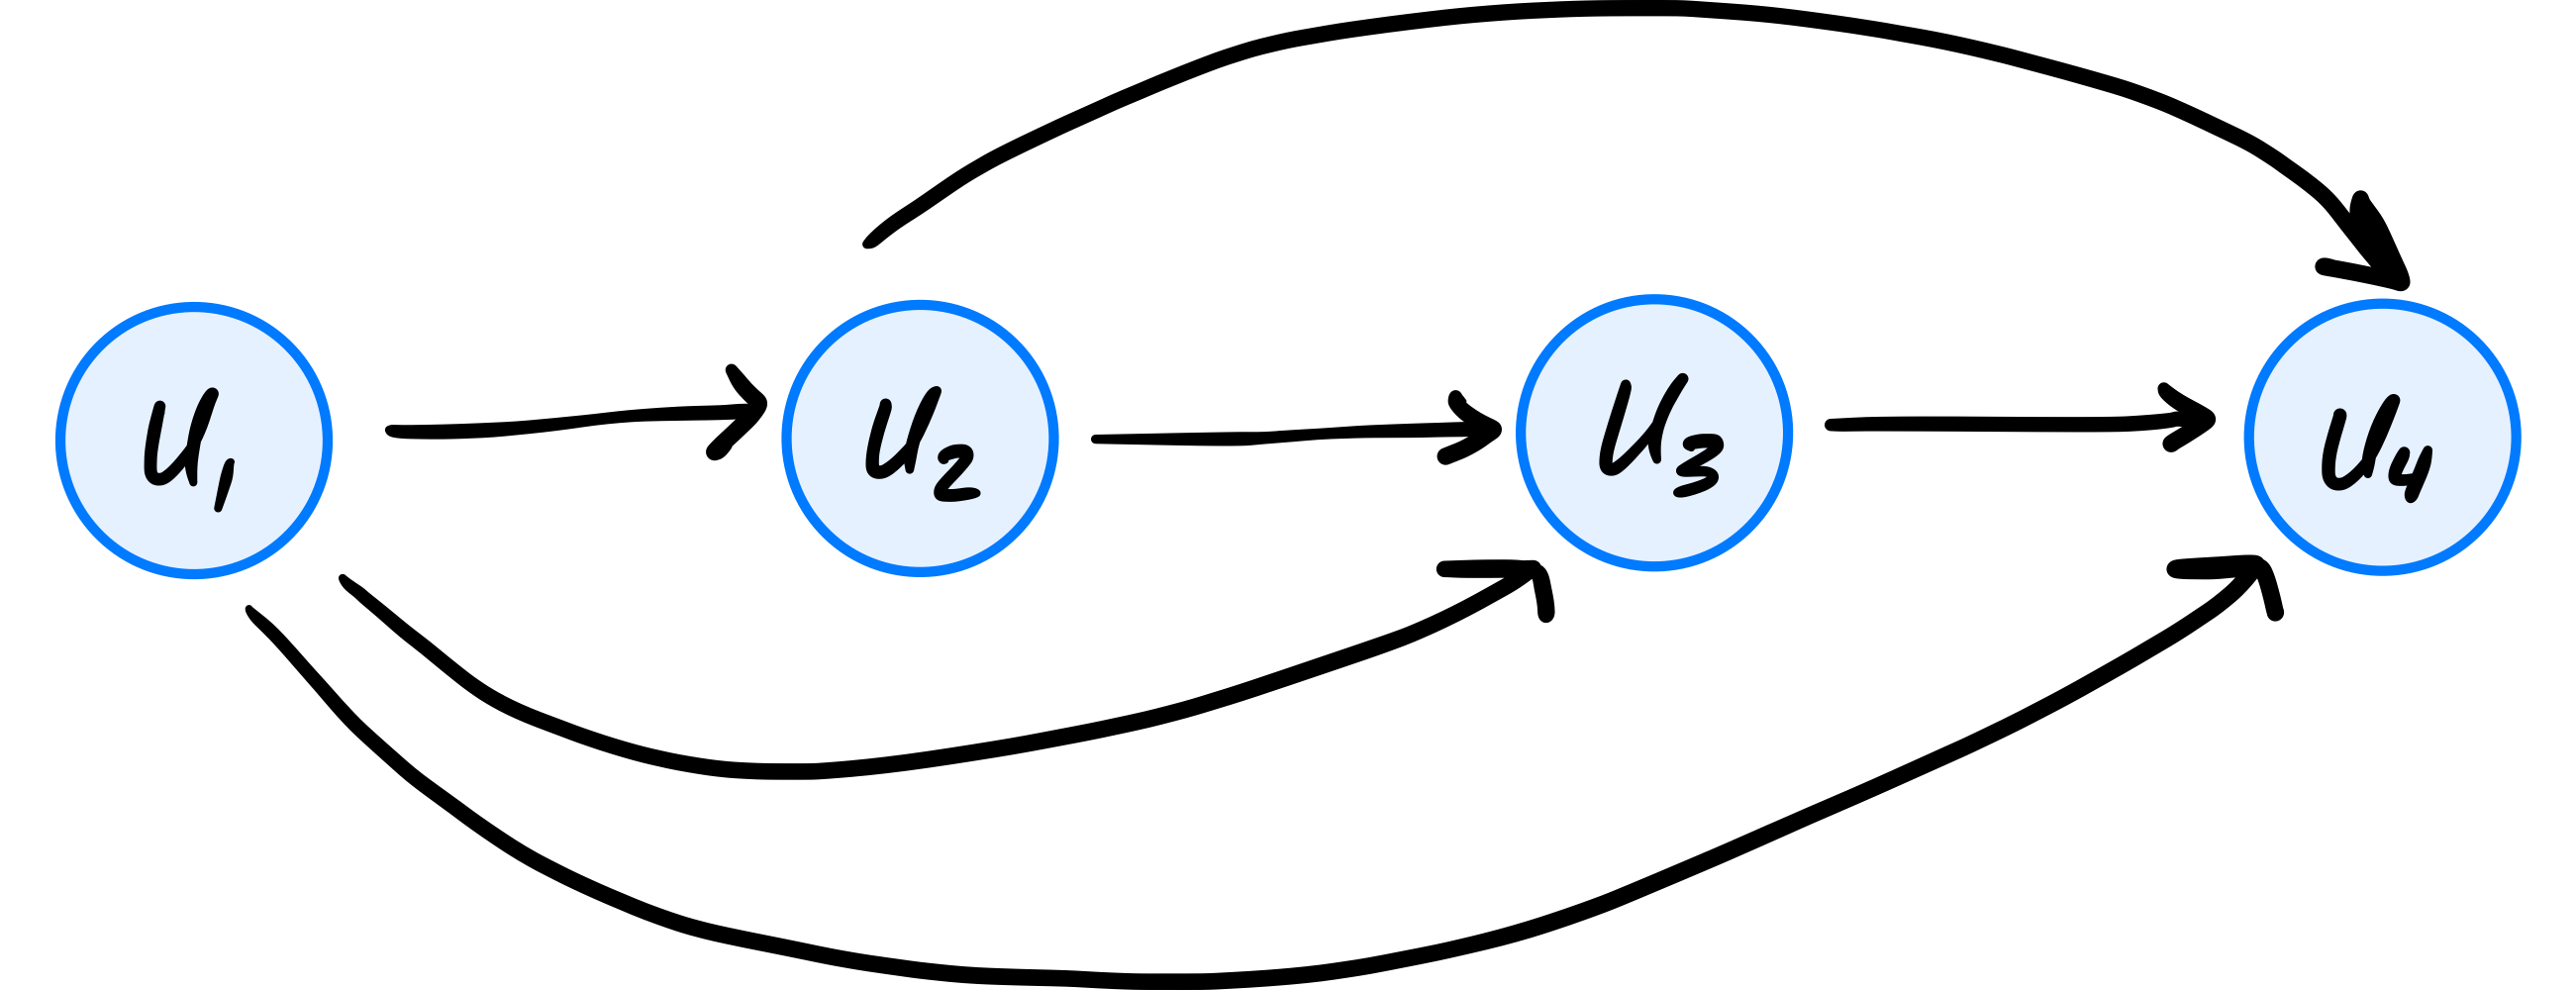
\includegraphics{./graph.png}

    What is the time complexity of depth-first search when run on a
    forward-looking graph with $n$ nodes, using node $u_1$ as the source? State
    your answer as a function of $n$ using asymptotic notation.

    \begin{soln}
        $\Theta(n^2)$
    \end{soln}

\end{prob}
